\section{Hadoop}
I big data sono un'industria a sé ma sono anche al centro delle strategie di molte aziende che desiderano migliorare la gestione dei clienti, il marketing e lo sviluppo. É quando si considerano campi dove la quantità di informazioni che girano intorno ad essi è così estesa, che entrano in gioco i sistemi distribuiti e strumenti come Hadoop che sono essenziali per gestire un notevole afflusso di dati. Proprio per questo motivo, in questa tesi, alla base del sistema distribuito implementato all'interno del progetto, c'è proprio Apache Hadoop. 
\subsection{Cosa è Hadoop}
Hadoop\footnote{Apache Hadoop: \href{https://hadoop.apache.org/}{https://hadoop.apache.org/}} è stato creato dalla Apache Software Foundation\footnote{Apache Software Foundation \href{https://www.apache.org/}{https://www.apache.org/}} ed è stato prodotto nei primi anni 2000 per rispondere alla crescita dei motori di ricerca come Yahoo e Google. Nato da Doug Cutting e Michael Cafarella, il progetto prese il nome dall'elefante giocattolo di uno degli sviluppatori. Hadoop è stato rilasciato come progetto open-source nel 2008 e poi nel 2012 dalla Apache Software Foundation. Oggi, Hadoop è composto da librerie open-source destinate ad elaborare grandi insiemi di dati su migliaia di computer in cluster.

Si tratta di un framework per l'esecuzione di applicazioni su grandi cluster costruiti con hardware di largo consumo a basso costo. Hadoop fornisce in modo trasparente applicazioni sia per l'affidabilità che per il trasferimento dei dati e consiste di quattro moduli principali:
\begin{itemize}
    \item \textbf{Hadoop Common}: utilities che supportano gli altri moduli Hadoop.
    \item \textbf{Hadoop Yet Another Resource Negotiator (YARN)}: Un framework per lo scheduling dei job e la gestione delle risorse del cluster
    \item \textbf{Hadoop Distributed File System (HDFS)}: Un file system distribuito che fornisce un accesso ad alta velocità ai dati delle applicazioni.
    \item \textbf{Hadoop MapReduce}: Un sistema basato su YARN per l'elaborazione parallela di grandi insiemi di dati.
\end{itemize}

Nella fase di sperimentazione, Hadoop è stato utilizzato per implementare un file system distribuito attraverso il quale, le macchine appartenenti al cluster possono processare i dataset di addestramento e di test in maniera distribuita. Per chiarire questo concetto abbiamo però bisogno di introdurre il funzionamento di HDFS, MapReduce e YARN.
\subsection{Hadoop Distributed File System} \label{hdfs}
L'Hadoop Distributed File System (HDFS)\footnote{Documentazione HDFS: \href{https://hadoop.apache.org/docs/r1.2.1/hdfs\_user\_guide.html}{https://hadoop.apache.org/docs/r1.2.1/hdfs\_user\_guide.html}} è un file system gerarchicho e distribuito progettato per funzionare su hardware di base. Ha molte somiglianze con i file system distribuiti esistenti. Tuttavia, le differenze con essi sono significative. HDFS è altamente tollerante agli errori ed è progettato per essere implementato su hardware a basso costo. Inoltre, fornisce un accesso ad alta velocità ai dati delle applicazioni ed è adatto al i software che utilizzano grandi set di dati.

L'architettura di HDFS è di tipo master/slave composta da un singolo master (\textbf{NameNode}) e un numero arbitrario di slaves/workers (\textbf{DataNode}), solitamente uno per ogni nodo del cluster. HDFS espone un namespace del file system e permette ai dati dell'utente di essere memorizzati in file, i quali sono divisi in uno o più blocchi che verranno memorizzati in un insieme di DataNodes. 

Il NameNode è un master server che possiede l'albero di tutte le directory del filesystem e gestisce operazioni di apertura, rinominazione e chiusura dei file. Risponde alla richiesta del client restituendo una lista di server DataNode pertinenti dove risiedono i dati. Qualsiasi cambiamento al namespace del file system o alle sue proprietà viene registrato dal NameNode. 

I DataNode contengono multipli blocchi di dati e la loro responsabilità è quella di eseguire operazioni di creazione, eliminazione e replicazione dei blocchi sotto istruzioni del NameNode. Una volta che il NameNode fornisce la posizione dei dati, le applicazioni client possono parlare direttamente con un DataNode mentre, replicando i dati, le istanze DataNode possono parlare tra loro.

Per garantire una buona tolleranza ai guasti, i blocchi di un file vengono replicati. La dimensione del blocco e il fattore di replica sono configurabili per ogni file e un'applicazione può specificare il numero di repliche al momento della sua creazione o cambiarlo in seguito.
\begin{figure}[hbt!]
    \centering
    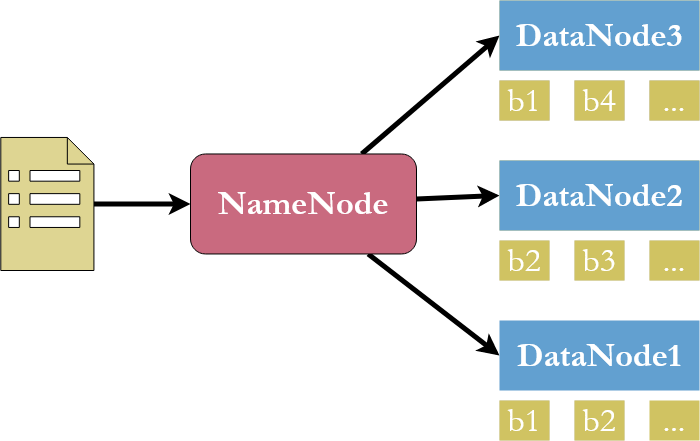
\includegraphics[width=0.7\textwidth]{img/hdfs.png}
    \caption{Architettura HDFS}
    \label{fig:hdfs_architettura}
\end{figure}

\subsection{MapReduce}
MapReduce\footnote{Documentazione MapReduce \href{https://hadoop.apache.org/docs/r1.2.1/mapred\_tutorial.html}{https://hadoop.apache.org/docs/r1.2.1/mapred\_tutorial.html}} è un framework per la creazione di applicazioni in grado di elaborare grandi quantità di dati in parallelo, permettendo una scalabilità massiccia su centinaia o migliaia di server in un cluster Hadoop. É stato reso popolare come modello di programmazione nel 2004 da Jeffery Dean e Sanjay Ghemawat di Google. Nel loro articolo \textit{MapReduce: simplified data processing on large clusters}\textsuperscript{\cite{pub62_mapreduce}} hanno discusso l'approccio di Google alla raccolta e all'analisi dei dati dei siti web per l'ottimizzazione della ricerca. Successivamente implementato da Apache, è diventato uno dei componenti principali del progetto Hadoop, nel quale, come il componenente HDFS è il responsabile della memorizzazione dei file, MapReduce si occupa di processare questi ultimi.

L'algoritmo implementato prende il nome dalle principali funzioni da cui è composto:
\begin{itemize}
    \item \textbf{Map}: trasforma i dati ricevuti in input in tuple formate da coppie chiave/valore.
    \item \textbf{Reduce}: prende in input l'output generato da Map e combina le coppie chiave-valore in un insieme più piccolo di tuple.
\end{itemize}
Tra le funzioni Map e Reduce avvengono operazioni di \textit{sorting} e \textit{shuffling} che si occupano di ordinare e raggruppare per chiave l'output di Map e fornirlo come input a Reduce.

MapReduce lavora secondo il principio del \textit{divide et impera}, suddividendo l'operazione di calcolo in diverse parti che verranno processate in modo autonomo per poi ricomporle (o ridurle) in un unico risultato finale. Queste parti sono dette \textit{jobs} e sono formate da sorgente di input, destinazione dei dati e le funzioni Map e Reduce.

Generalmente, l'algoritmo viene eseguito sugli stessi nodi su cui risiede HDFS, il che significa che ognuno di essi viene utilizzato sia per il calcolo che per lo storage. Il vantaggio di una tale configurazione è che i compiti possono essere programmati sui nodi dove risiedono i dati e quindi risulta un'elevata larghezza di banda aggregata in tutto il cluster.
\begin{figure}[hbt!]
    \centering
    \includegraphics[width=1\textwidth]{img/mapreduce.png}
    \caption{Algoritmo MapReduce}
    \label{fig:mapreduce}
\end{figure}\\

Come e da chi vengono gestite internamente queste operazioni? MapReduce, a livello architetturale, presenta due componenti: 
\begin{itemize}
    \item \textbf{Job Tracker}: si occupa della gestione delle risorse (CPU e memoria) e del ciclo di vita di un job MapReduce. Il JobTracker distribuisce il lavoro tra i nodi più vicini che contengono i dati da elaborare; nel caso in cui un nodo non possa ospitare il task, si fa poi carico della schedulazione del job nonché della ripetizione dell’esecuzione dei singoli task di MapReduce che si trovano in uno stato di errore. 
    \item \textbf{Task Tracker}: Sono le componenti che girano sui singoli nodi e che eseguono effettivamente i task sotto la direzione del JobTracker.
\end{itemize}

Cosa rende questo framework così importante? I benefici che porta sono notevoli e, alla sua nascita, portò grande innovazione nel campo del calcolo distribuito. I due principali vantaggi che questa tecnologia offre sono:
\begin{enumerate}
    \item \textbf{Elaborazione parallela}: l'intero lavoro è diviso in job che vengono elaborati in modo parallelo simultaneamente, riducendo drasticamente i tempi di esecuzione.
    \item \textbf{Località dei dati}: invece di spostare tutti i dati per l'elaborazione, il processo completo viene spostato su ogni nodo. Col crescere del quantitativo di dati da processare, può diventare difficile spostarli da un posto all'altro e quindi questa tecnica è considerata un'alternativa assai vantaggiosa.
\end{enumerate}


\subsection{YARN} \label{yarn}
Quando i dati hanno cominciato a diventare sempre più grandi, Hadoop File System è stato in grado di immagazzinarli, ma MapReduce è diventato un collo di bottiglia nelle prestazioni. Questo perché, in Hadoop 1.x, il JobTracker si occupava sia della gestione delle risorse, sia dell'elaborazione dei dati. Per questo motivo, in Hadoop 2.0\footnote{Hadoop 2.0 changelog: \href{https://hadoop.apache.org/release/2.2.0.html}{https://hadoop.apache.org/release/2.2.0.html}} è stato introdotto \textit{YARN\footnote{YARN docs: \href{https://hadoop.apache.org/docs/current/hadoop-yarn/hadoop-yarn-site/YARN.html}{https://hadoop.apache.org/docs/current/hadoop-yarn/hadoop-yarn-site/YARN.html}} (Yet Another Resources Navigator)} che separa il livello di gestione delle risorse dal livello di elaborazione. L'idea fondamentale di YARN è di dividere queste funzionalità in processi separati:
\begin{itemize}
    \item \textbf{ResourceManager}: è il processo master di YARN ed è responsabile dell'assegnazione e della gestione delle risorse tra tutte le applicazioni. Ogni volta che riceve una richiesta di elaborazione, la inoltra al gestore del nodo corrispondente (NodeManager) e alloca le risorse per il completamento della richiesta. Viene suddiviso in ulteriori due componenti:
    \begin{itemize}
        \item \textbf{Scheduler}: esegue la pianificazione in base all'applicazione assegnata e alle risorse disponibili. Non esegue altri compiti come il monitoraggio o il tracking e non garantisce un riavvio se un compito fallisce. 
        \item \textbf{ApplicationManager}: è responsabile di dell'accettazione dell'applicazione e della negoziazione del primo container\footnote{Per container si intende un insieme di risorse fisiche come RAM, core di CPU e disco su un singolo nodo.} dal gestore delle risorse. Riavvia anche il container ApplicationMaster se un job fallisce.
    \end{itemize}
    \item \textbf{NodeManager}: è l'agente del framework per ogni macchina ed è responsabile del monitoraggio del loro utilizzo delle risorse (cpu, memoria, disco, rete) e della segnalazione al ResourceManager. Si registra con il ResourceManager e invia \textit{heartbeat} (segnali) con lo stato di salute del nodo. Monitora l'uso delle risorse, esegue la gestione dei log e uccide anche un container in base alle indicazioni del gestore delle risorse. 
    \item \textbf{ApplicationMaster}: è una libreria specifica del framework e ha il compito di negoziare le risorse dal ResourceManager e lavorare con i NodeManager per eseguire e monitorare i job.
\end{itemize}

\begin{figure}[ht!]
    \centering
    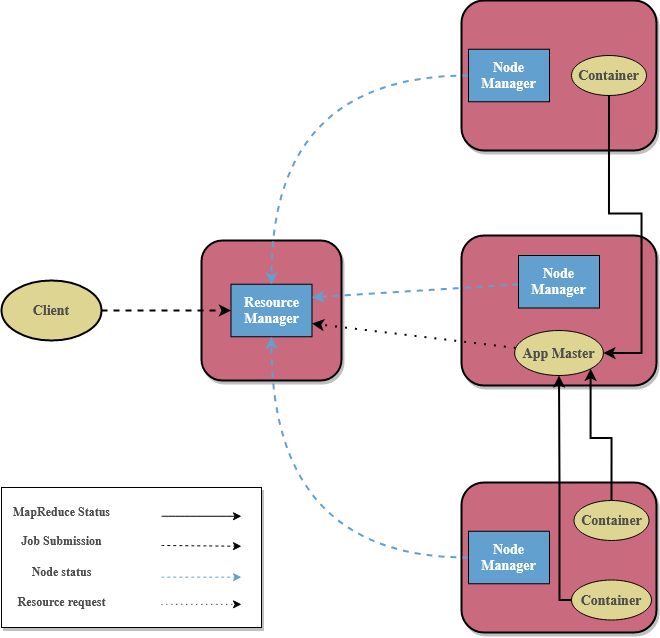
\includegraphics[width=0.8\textwidth]{img/yarn.png}
    \caption{Architettura YARN}
    \label{fig:yarn}
\end{figure}
\clearpage
%  \subsection{Utilizzo di Hadoop} \label{uso_hadoop}
Descritte le componenti HDFS e MapReduce, è possibile proseguire con illustrando come Hadoop è stato inserito all’interno del progetto di Tesi.

Come citato precedentemente, l’obiettivo ultimo è quello di testare soluzioni per la risoluzione di task di NLP in ambiente distribuito. Per fare ciò è stato configurato un database distribuito HDFS su di un cluster di 3 macchine connesse tre loro. Così facendo, tutte le macchine del sistema hanno accesso ai file contenenti i dataset di addestramento e di testing, ed ai modelli utilizzati (sia preaddestrati che allenati al momento della sperimentazione). Nel dettaglio, il nodo master del cluster ospita il NameNode, che si occupa della gestione del namespace del file system, mentre su ognuna delle altre macchine è stato invece allocato un processo DataNode, con lo scopo di delegare loro la manipolazione dei blocchi di dati secondo le indicazioni del NameNode.

Il concetto di MapReduce è invece ereditato da Apache Spark, framework su cui si basa Spark NLP, ovvero il soggetto di questo lavoro. Spark, come avviene con MapReduce, suddivide il processo in jobs e distribuisce questi ultimi tra i nodi del cluster migliorando le proprie prestazioni in fatto di distribuzione del carico e velocità di esecuzione. Nel capitolo successivo si entrerà nel dettaglio del funzionamento di Spark e di come è stato implementato all’interno del progetto.